% Figure 1: T2T vs T2M overview
% Colours defined here for Overleaf compatibility
\definecolor{cOkFill}{HTML}{E8F5E9}
\definecolor{cOkBord}{HTML}{4CAF50}
\definecolor{cErrFill}{HTML}{FFEBEE}
\definecolor{cErrBord}{HTML}{E57373}
\definecolor{cMskFill}{HTML}{EEEEEE}
\definecolor{cMskBord}{HTML}{9E9E9E}
\definecolor{cFixFill}{HTML}{E3F2FD}
\definecolor{cFixBord}{HTML}{42A5F5}
\definecolor{cRedTitle}{HTML}{C62828}
\definecolor{cBlueTitle}{HTML}{1565C0}
\definecolor{cRedDark}{HTML}{B71C1C}
\definecolor{cBlueDark}{HTML}{0D47A1}
\definecolor{cGreen}{HTML}{2E7D32}
\definecolor{cGrey}{HTML}{888888}

\begin{figure}[t]
\centering
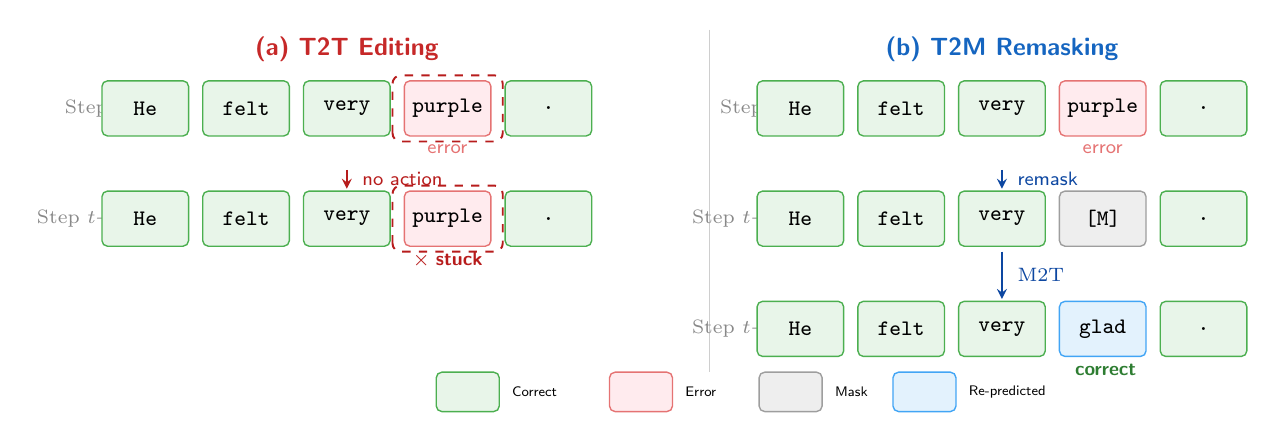
\begin{tikzpicture}[
  % token boxes
  tok/.style={draw, rounded corners=2pt, minimum height=7mm, minimum width=11mm,
              font=\footnotesize\ttfamily, inner sep=2pt, line width=0.5pt},
  ok/.style ={tok, fill=cOkFill,  draw=cOkBord},
  err/.style={tok, fill=cErrFill, draw=cErrBord},
  msk/.style={tok, fill=cMskFill, draw=cMskBord},
  fix/.style={tok, fill=cFixFill, draw=cFixBord},
  % labels
  steplbl/.style={font=\scriptsize, text=cGrey},
  tag/.style={font=\scriptsize\sffamily},
  arr/.style={->, >=stealth, line width=0.6pt},
  panel/.style={font=\small\bfseries\sffamily},
]

% horizontal / vertical spacing
\pgfmathsetmacro{\dx}{1.28}
\pgfmathsetmacro{\dy}{1.4}
\pgfmathsetmacro{\xstart}{0}

% =====================================================================
%  (a) T2T Editing — left
% =====================================================================
\begin{scope}[shift={(0,0)}]

  \node[panel, text=cRedTitle] at (2*\dx, 0.75) {(a) T2T Editing};

  % Step t
  \node[steplbl, anchor=east] at (\xstart-0.15, 0) {Step $t$};
  \foreach \i/\w/\s in {0/He/ok, 1/felt/ok, 2/very/ok, 3/purple/err, 4/./ok} {
    \node[\s] at (\xstart+\i*\dx, 0) {\w};
  }
  \node[tag, text=cErrBord] at (\xstart+3*\dx, -0.52) {\textsf{error}};

  % arrow
  \draw[arr, cRedDark] (\xstart+2*\dx, -0.78) -- (\xstart+2*\dx, -\dy+0.38)
    node[midway, right=2pt, tag, text=cRedDark] {no action};

  % Step t+1
  \node[steplbl, anchor=east] at (\xstart-0.15, -\dy) {Step $t{+}1$};
  \foreach \i/\w/\s in {0/He/ok, 1/felt/ok, 2/very/ok, 3/purple/err, 4/./ok} {
    \node[\s] at (\xstart+\i*\dx, -\dy) {\w};
  }
  \node[tag, text=cRedDark, font=\scriptsize\sffamily\bfseries]
    at (\xstart+3*\dx, -\dy-0.52) {$\times$\;\textsf{stuck}};

  % dashed highlight on the stuck error token
  \draw[dashed, cRedDark, line width=0.7pt, rounded corners=3pt]
    (\xstart+3*\dx-0.7, 0-0.42) rectangle (\xstart+3*\dx+0.7, 0+0.42);
  \draw[dashed, cRedDark, line width=0.7pt, rounded corners=3pt]
    (\xstart+3*\dx-0.7, -\dy-0.42) rectangle (\xstart+3*\dx+0.7, -\dy+0.42);

\end{scope}

% =====================================================================
%  Vertical divider
% =====================================================================
\draw[cMskBord!50, line width=0.4pt] (5.6*\dx, 1.0) -- (5.6*\dx, -3.35);

% =====================================================================
%  (b) T2M Remasking — right
% =====================================================================
\begin{scope}[shift={(6.5*\dx, 0)}]

  \node[panel, text=cBlueTitle] at (2*\dx, 0.75) {(b) T2M Remasking};

  % Step t
  \node[steplbl, anchor=east] at (\xstart-0.15, 0) {Step $t$};
  \foreach \i/\w/\s in {0/He/ok, 1/felt/ok, 2/very/ok, 3/purple/err, 4/./ok} {
    \node[\s] at (\xstart+\i*\dx, 0) {\w};
  }
  \node[tag, text=cErrBord] at (\xstart+3*\dx, -0.52) {\textsf{error}};

  % arrow: remask
  \draw[arr, cBlueDark] (\xstart+2*\dx, -0.78) -- (\xstart+2*\dx, -\dy+0.38)
    node[midway, right=2pt, tag, text=cBlueDark] {remask};

  % Step t+1: remasked
  \node[steplbl, anchor=east] at (\xstart-0.15, -\dy) {Step $t{+}1$};
  \foreach \i/\w/\s in {0/He/ok, 1/felt/ok, 2/very/ok, 3/{[M]}/msk, 4/./ok} {
    \node[\s] at (\xstart+\i*\dx, -\dy) {\w};
  }

  % arrow: M2T
  \draw[arr, cBlueDark] (\xstart+2*\dx, -\dy-0.42) -- (\xstart+2*\dx, -2*\dy+0.38)
    node[midway, right=2pt, tag, text=cBlueDark] {\textrm{M2T}};

  % Step t+2: corrected
  \node[steplbl, anchor=east] at (\xstart-0.15, -2*\dy) {Step $t{+}2$};
  \foreach \i/\w/\s in {0/He/ok, 1/felt/ok, 2/very/ok, 3/glad/fix, 4/./ok} {
    \node[\s] at (\xstart+\i*\dx, -2*\dy) {\w};
  }
  \node[tag, text=cGreen, font=\scriptsize\sffamily\bfseries]
    at (\xstart+3*\dx, -2*\dy-0.52) {$\checkmark$\;\textsf{correct}};

\end{scope}

% =====================================================================
%  Legend (centred at bottom)
% =====================================================================
\begin{scope}[shift={(3.2*\dx, -3.6)}]
  \node[ok,  minimum width=8mm, minimum height=5mm] (L1) at (0,0) {};
  \node[font=\tiny\sffamily, anchor=west] at (L1.east) {\,Correct};
  \node[err, minimum width=8mm, minimum height=5mm] (L2) at (2.2,0) {};
  \node[font=\tiny\sffamily, anchor=west] at (L2.east) {\,Error};
  \node[msk, minimum width=8mm, minimum height=5mm] (L3) at (4.1,0) {};
  \node[font=\tiny\sffamily, anchor=west] at (L3.east) {\,Mask};
  \node[fix, minimum width=8mm, minimum height=5mm] (L4) at (5.8,0) {};
  \node[font=\tiny\sffamily, anchor=west] at (L4.east) {\,Re-predicted};
\end{scope}

\end{tikzpicture}
\caption{\textbf{\TtoT{} editing vs.\ \TtoM{} remasking.}
Both panels start from the same state where the erroneous token ``purple'' has been committed at position~4.
\textbf{(a)}~\TtoT{} detects the error but cannot correct it:
the conditional distribution is multimodal (``happy,'' ``glad,'' ``pleased'' each receive ${\sim}0.25$ probability),
so no single candidate exceeds the confidence threshold $\tau_{\text{t2t}}$---the error remains in place (\emph{correction inertia}), polluting context for all subsequent predictions.
\textbf{(b)}~\TtoM{} detects the same error via low posterior probability ($p_\theta(\text{``purple''}) = 0.02 \ll \tau_{\text{lp}}$) and resets the position to \mask{}, removing the adversarial signal from context (\emph{context purification}).
A subsequent \MtoT{} step re-predicts the position under cleaner context and produces the correct token ``glad'' (\emph{delayed commitment}).}
\label{fig:overview}
\end{figure}
